\chapter{\emph{Improving the Quality of Experience}: Engineering High Quality Untethered Multi-user VR for Commodity Mobile Devices} \label{chap:vr}



\section{Introduction}
Virtual Reality (VR) has registered numerous applications. In
this chapter, we focus on multi-user VR where multiple users
jointly participate in exploring a VR scene. This enables
many applications that single-user VR cannot support such as
team training, social VR, group therapy, collaborative product
design, and multi-user gaming.

We envision the following use case with more than 10 collocated users in a VR room. To start multi-user VR, each user simply launches the app on her smartphone and plugs the phone into a VR headset (\eg a \$50 Samsung Gear VR~\cite{samsung-gear-vr} or even a \$10 Google Cardboard~\cite{google-cardboard} with a \$6 VR controller~\cite{vr-controller}).
These mobile devices fetch the VR content from an off-the-shelf server based on the users' real-time motion. The devices and the server communicate wirelessly over a single WiFi access point (AP). The users can enjoy the high-quality VR content as if it is rendered by a desktop PC with a powerful GPU. Meanwhile, each user can see and possibly interact with other users in the virtual world.

My work therefore aims at realizing the above ambitious use case. We design \firefly, a novel multi-user VR system for mobile devices. The  goals of \firefly are the following.
First, \firefly works with affordable, commercial off-the-shelf (COTS) mobile devices, server, and AP. This helps reduce the deployment cost and facilitate the ``bring-your-own-device'' (BYOD) policies that many enterprises adopt today~\cite{byodref}.
Second, \firefly employs untethered, wireless VR to overcome the inconvenience and trip hazards incurred by wired cables~\cite{triphazard}. This is important for multi-user VR where multiple users' cables may easily get intertwined.
Third, \firefly offers high content quality, low ``motion-to-photon'' (M2P) latency, and high frame rate. An M2P higher than 16ms may cause nausea to VR users~\cite{motionsickness}. We target Quad HD (1440p) resolution, 60 frames per second (FPS) that can provide a good experience even for fast-paced VR gaming -- the most demanding VR task~\cite{vr_gaming}.
Fourth, \firefly aims at supporting $\sim$15 users who can form a sizeable group of, for example, co-workers, students, and patients. To the best of our knowledge, no existing system can achieve this using a single commodity server and WiFi AP. 
Fifth, \firefly allows complex VR scenes with both background and dynamic foreground objects, such as other users' avatars that users can interact with.

The above goals pose tremendous challenges. The CPU/GPU power of a smartphone is at least one order of magnitude lower than its desktop counterpart~\cite{satyanarayanan2019computing}, not to mention the energy/heat constraints;
the heterogeneity of their computational capabilities should also to be taken into consideration;
the bandwidth offered by a single AP is limited for multiple users;
another key challenge is multi-user scalability, which calls for strategic decisions of splitting the client-server workload,
as well as scalable approaches for rendering and distributing the content.
To address the above challenges, \firefly makes a series of judicious design decisions as follows.

\BULLET \firefly performs one-time, offline content preparation by enumerating, pre-rendering, and storing
the views at all positions reachable in a virtual scene. At runtime, given a user's position and viewing direction, the server directly retrieves the stored high-quality content and delivers it to the user. This completely eliminates the online rendering overhead.
Prior work~\cite{boos2016flashback} applies offline rendering to a single mobile device for local VR scenes, while \firefly further extends this concept to networked multi-user VR where offline rendering is found to be an indispensable mechanism ensuring scalability.

\BULLET To reduce the network bandwidth consumption, \firefly takes a viewport-adaptive approach: each user only requests for the content that the user is about to perceive based on motion prediction.
We conduct a thorough analysis of 25 human users' motion traces collected from an IRB-approved user trial.
The results shed light on developing a lightweight yet effective motion prediction approach for \firefly.
%In the literature, several studies~\cite{fan2017fixation,hou2018predictive,bao2016shooting} have examined 360\degree{} video viewers' viewing patterns that only involve rotational movement (yaw and pitch). Our study instead investigates generic VR users' motion that consists of both the rotational and translational viewport movement as well as their interplay (\S\ref{sec:??}).% move this to related work

\BULLET \firefly supports \emph{Adaptive Quality Control (AQC)}, which determines the content quality of each user based on the total network bandwidth, the bandwidth available to each user, and the amount of to-be-delivered content.
AQC essentially extends traditional video bitrate adaptation~\cite{jiang2012improving,huang2014buffer,yin2015control,mao2017neural}:
from handling a single client to multiple clients,
from dealing with regular videos to immersive VR content, and
from being invoked at the second level to the millisecond level to adapt to users' motion.
These differences require AQC to be effective, lightweight, fair, and scalable.

\BULLET \firefly handles dynamic foreground objects in a scalable and adaptive manner.
Specifically, objects' 3D models are distributed to the clients offline.
They are then rendered locally by the client. This eliminates the uncertainty caused by the network as well as the potential resource competition from other users compared to a server-side approach.
To prevent too many objects appearing in the viewport from slowing down client-side rendering, \firefly supports adaptively reducing the objects' fidelity to maintain a high FPS.

We are currently working on the full implementation of \firefly system, in the following part of this section we will discuss the design of \firefly, highlight preliminary results, and point out future works. 

\section{Firefly Overview}

\firefly server exhaustively enumerates all possible views at all positions, renders them at a high quality, encodes them into video frames, and saves the frames in the storage.
%
At runtime, the server simply retrieves and transmits the pre-encoded frames based on each user's position and viewport. In this way, the rendering/encoding overhead at runtime is completely eliminated, so the server can easily scale to tens or even hundreds of simultaneous users. These benefits come at the cost of high storage usage, which is largely not an issue given the cheap storage today.
%
Figure~\ref{fig:system_design} plots the overall architecture. As shown, \firefly consists of a content server and multiple commodity mobile devices. %such as a VR headset with a smartphone plugged in.
They are wirelessly connected through a WiFi access point (AP). This setup can be easily realized in enterprise or home environments at a very low cost.
%
Note that prior work~\cite{boos2016flashback} applies offline rendering to a single mobile device for local VR scenes, while \firefly further extends this concept to networked multi-user VR where offline rendering is found to be an indispensable mechanism ensuring the scalability.

\begin{figure}[t]
	\centering
	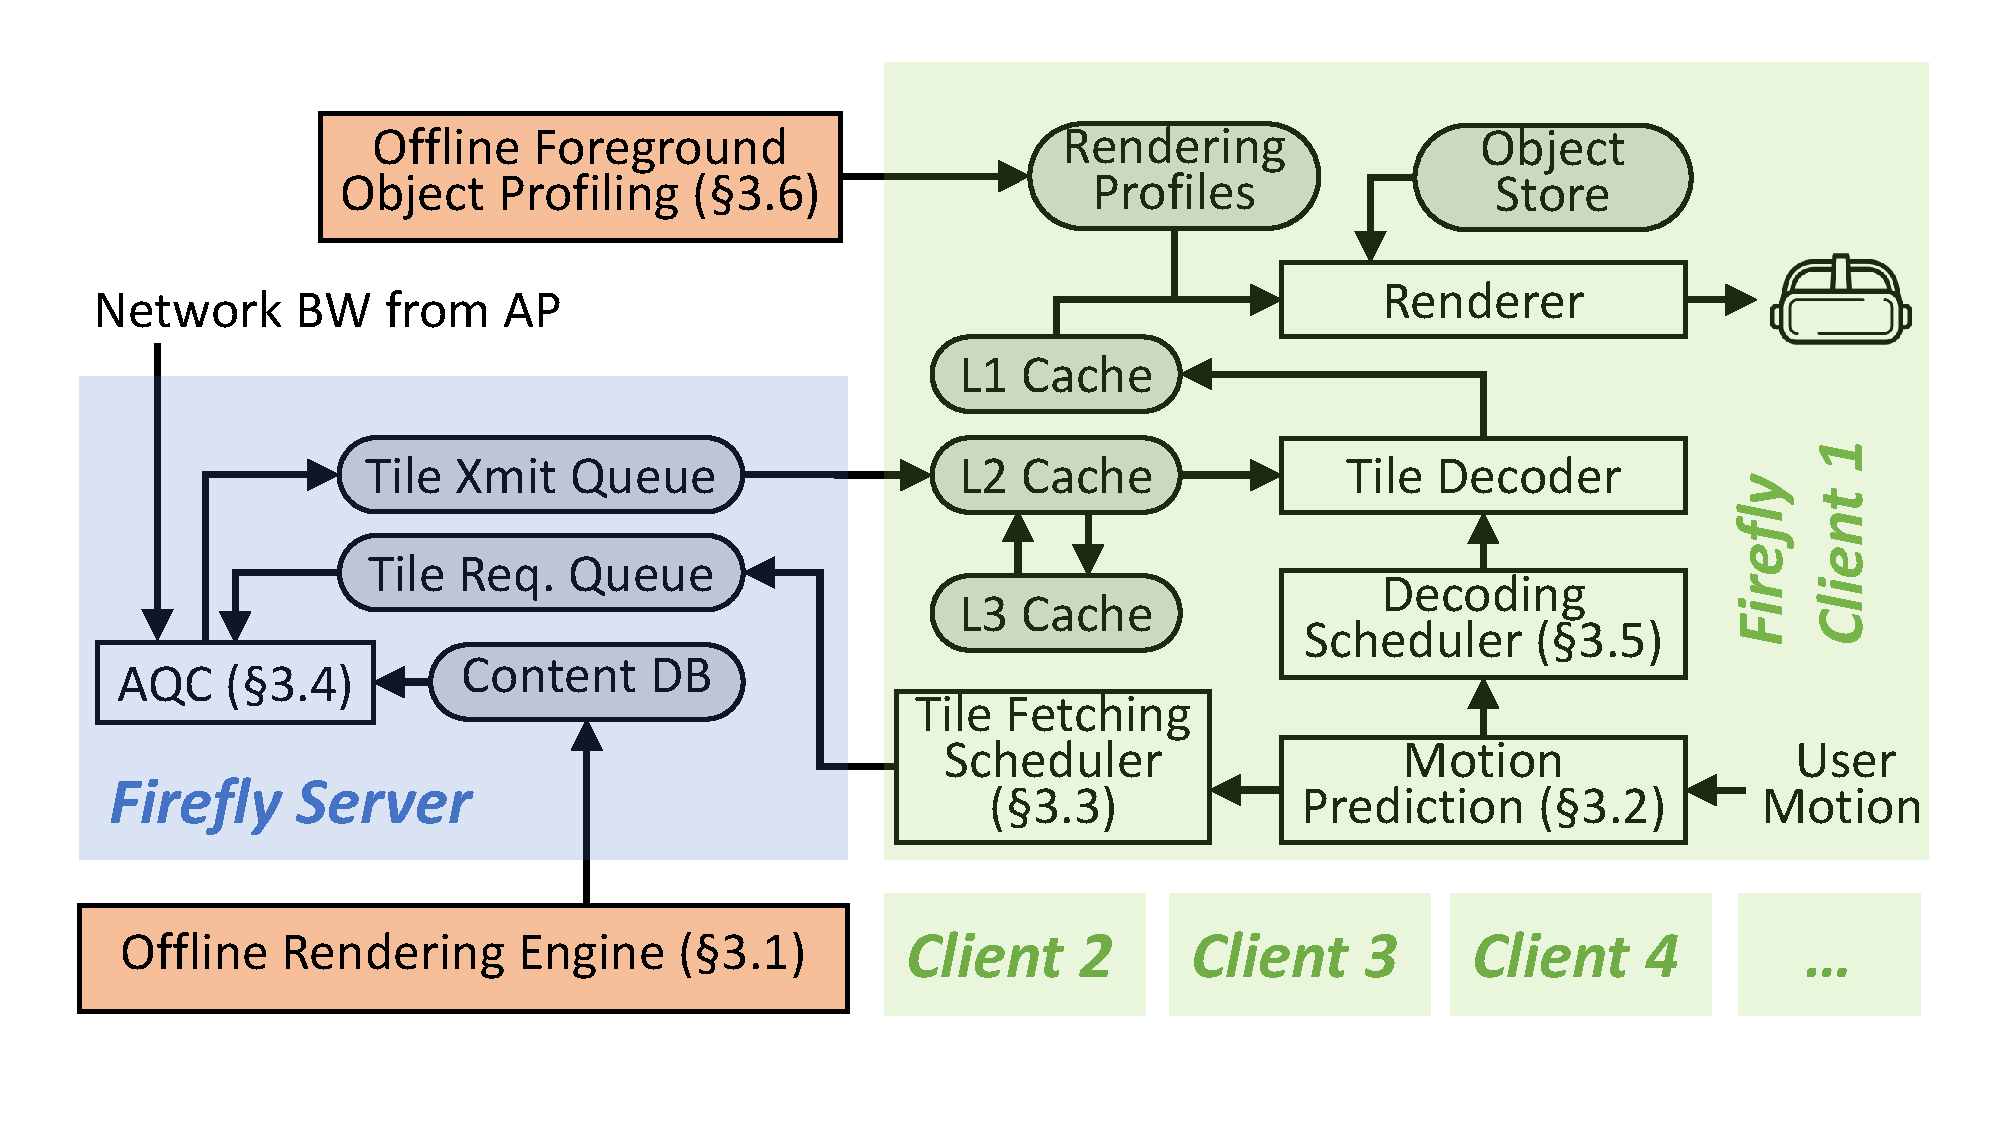
\includegraphics[width=.8\textwidth]{figs/firefly/arch.pdf}
	\caption{The \firefly system architecture.}
	\label{fig:system_design}
	\vspace{-.2in}
\end{figure}

The server consists of a content database that stores rendered/encoded content indexed by a user's position and viewing direction. The database is built by the Offline Rendering Engine that performs the aforementioned exhaustive content generation.
%
Another critical component is the AQC module that is introduced to scale the system and to handle the wireless bandwidth fluctuation. It determines in real-time the content quality for each user.
%
Designing AQC is challenging due to multiple requirements including boosting users' QoE, maintaining good performance, ensuring scalability, and achieving fairness.

On the client side, there are two high-level design choices on the content fetching strategy for background frames.
%on the client side.
First, the client can prefetch all surrounding frames at every new virtual position~\cite{lai2019furion}.
%similar to Furion~\cite{lai2019furion} scheme.
However, this technique may consume high bandwidth with a considerable amount of wasted traffic (\ie the fetched content is not viewed by the user), making it infeasible for multi-user VR.
%
Second, to reduce the bandwidth footprint, the client can use its historical motion trajectory to predict the future viewport and to
prefetch only the portions that will likely be consumed in the near future. \firefly is the first to incorporate this viewport-adaptative approach into generic VR using robust motion prediction (\S\ref{sec:motion_prediction}).
%The client also uses an efficient hierarchical cache management (\S\ref{sec:cache}).
The client also efficiently manages its local cache and handles foreground dynamic objects in an adaptive and scalable manner.

\begin{figure*}[t]
	\centering
	\begin{minipage}{.4\textwidth}
		\centering
		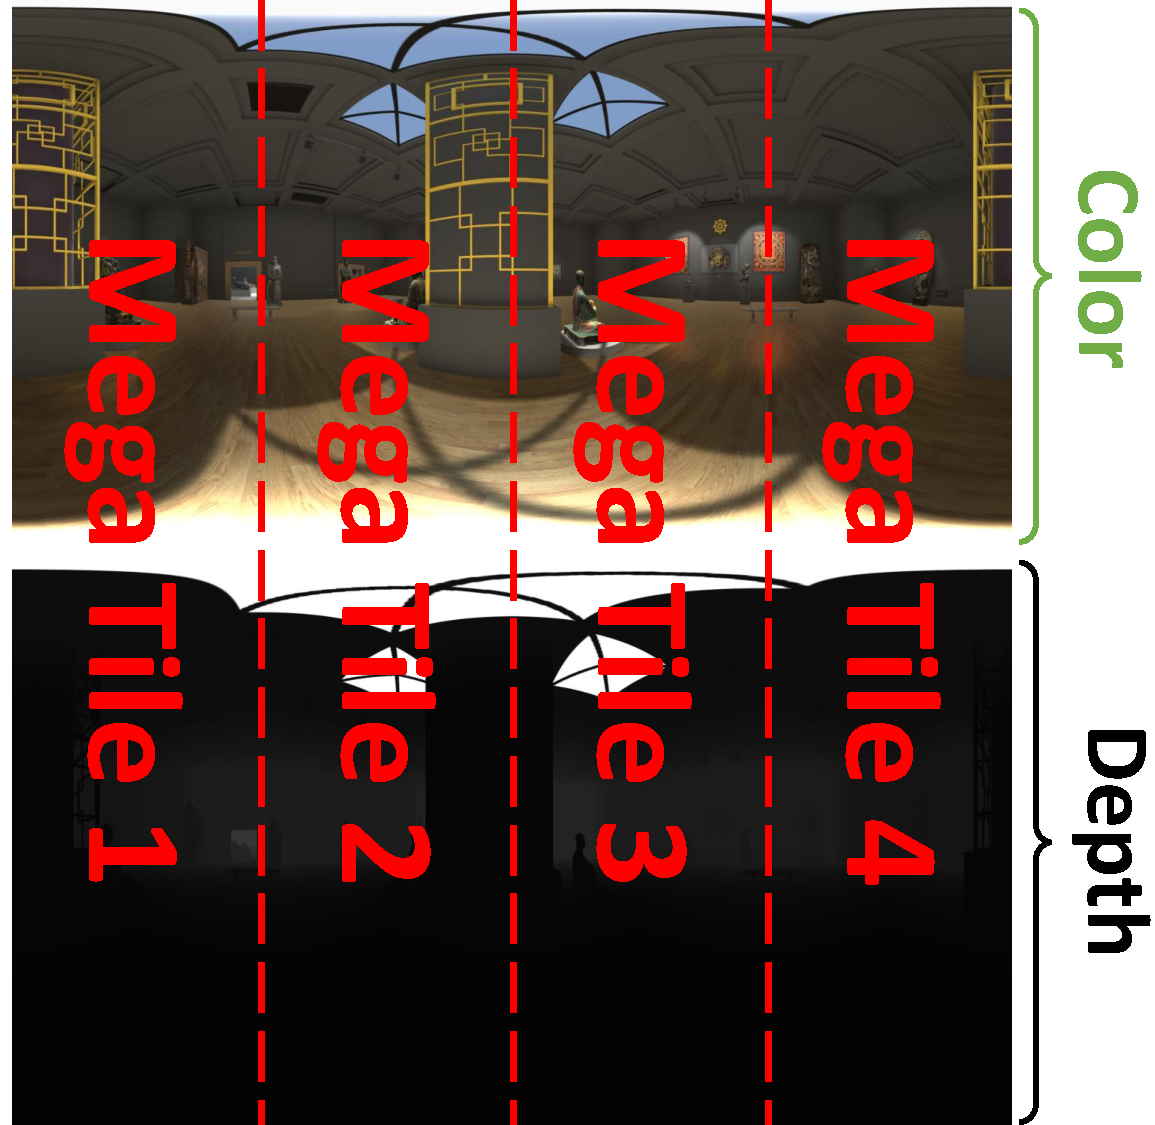
\includegraphics[width=\linewidth]{figs/firefly/MT.pdf}
		\vspace{-.1in}
		\caption{\small Mega frame.}
		\label{fig:mf}
	\end{minipage}
	\begin{minipage}{.5\textwidth}
		\centering
		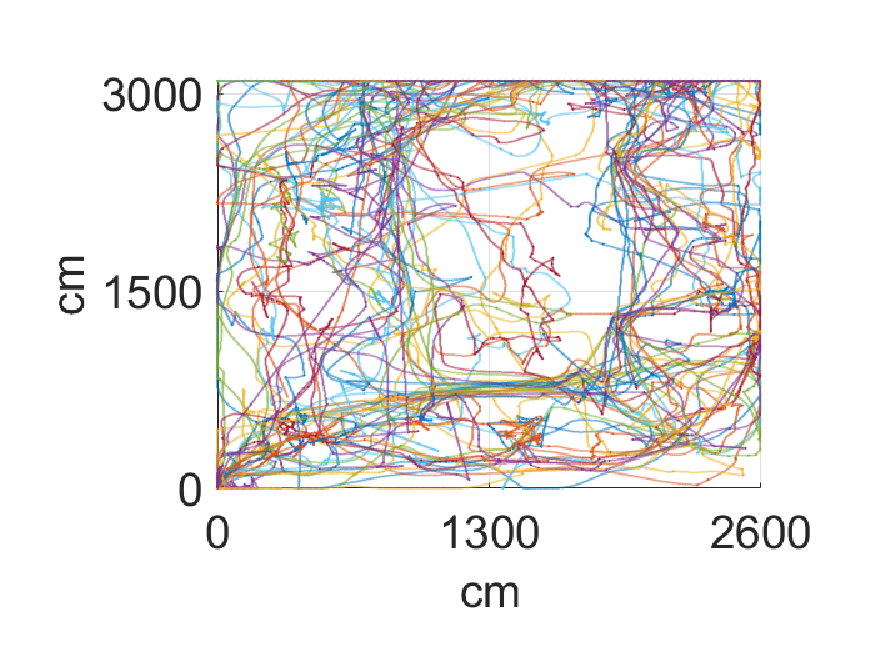
\includegraphics[width=\linewidth]{figs/firefly/office_trajectory.pdf} \vspace{-.25in}
		\caption{\small Users' translational trajectories (the Office scene).}
		\label{fig:office_trajectory}
	\end{minipage}
\end{figure*}

\subsection{Offline rendering engine}
The offline rendering engine produces the content database.
%The detailed content generation process is as follows.
%
The whole VR world is discretized into grids. At each grid position that the user can reach, the rendering engine renders a \emph{mega frame} that captures the 360\degree{} panoramic view that the user can possibly perceive at a high quality. \firefly uses Equirectangular projection~\cite{equirectangular} to generate the panoramic representation, but other projection algorithms~\cite{pyramid,cubemap,yu2015framework} can also be applied. As shown in Figure~\ref{fig:mf}, besides the color frame (top), a mega frame also includes a panoramic depth map (bottom) where the brightness of each pixel indicates its distance from the user. The depth map will be used to ensure the correct occlusion when overlaying foreground objects such as avatars of other users onto the scene. %In other words, a mega frame captures the panoramic 3D environment at each position.

We next apply the \emph{tiling} technique~\cite{qian2018flare,he2018rubiks} by dividing each mega frame into \emph{mega tiles}. Each tile is independently encoded and can be separately transmitted and decoded.
%
The rationale is that, since the user only sees a portion of the whole panoramic scene at a given time, there is oftentimes no need to fetch the entire mega frame. The mega tiles thus allow users to (pre)fetch the content more adaptively at a finer granularity, to reduce the network bandwidth consumption.
%
The tiling scheme requires the user to predict its viewport, \ie to determine which tiles to fetch based on the observed viewport trajectory.

A decision we need to make is to determine the number of tiles and their layout.
While having more tiles provides more bandwidth saving opportunities, in the meantime it increases the decoding overhead %\xing{we just mentioned it reduces decoding overhead}
and makes compression less efficient.
%The latter is because similar content falling into different tiles has to be separately encoded, incurring redundant data.
After carefully studying the above tradeoffs using real users' viewport trajectory data (\S\ref{sec:motion_prediction}), we decide to vertically segment each mega frame into four mega tiles as shown in Figure~\ref{fig:mf}. We choose vertical segmentation because according to our data collected from 25 users,
users tend to keep their sight vertically centered (\ie looking at the equator) while moving the viewport horizontally.
%
This makes horizontal segmentation at the equator (0\degree{} latitude) inefficient because the vertically centered viewport will always overlap with at least two tiles, \ie one above and the other below the equator.

As described above, at each position, the offline rendering engine renders four tiles capturing the panoramic view and depth. Each tile is then independently encoded into video frames with multiple quality levels.
%
The rendered and encoded tiles are stored in the content database, indexed by the user's grid position, the tile ID (1 to 4), and the quality level.


\section{VR Viewport Movement: Characterization and Prediction}
\label{sec:motion_prediction}

Users' motion makes VR immersive and interactive. In the literature, many studies have investigated users' head \emph{rotational} movement when watching 360\degree{} videos~\cite{fan2017fixation,hou2018predictive,bao2016shooting}. Generic VR differs from 360\degree{} videos in that it further involves \emph{translational} movement.
%
To our knowledge, no prior study has comprehensively investigated VR users' motion patterns and their predictability, which are our focus here.

\begin{figure*}[t]
	\centering
	\begin{minipage}{.45\textwidth}
		\centering
		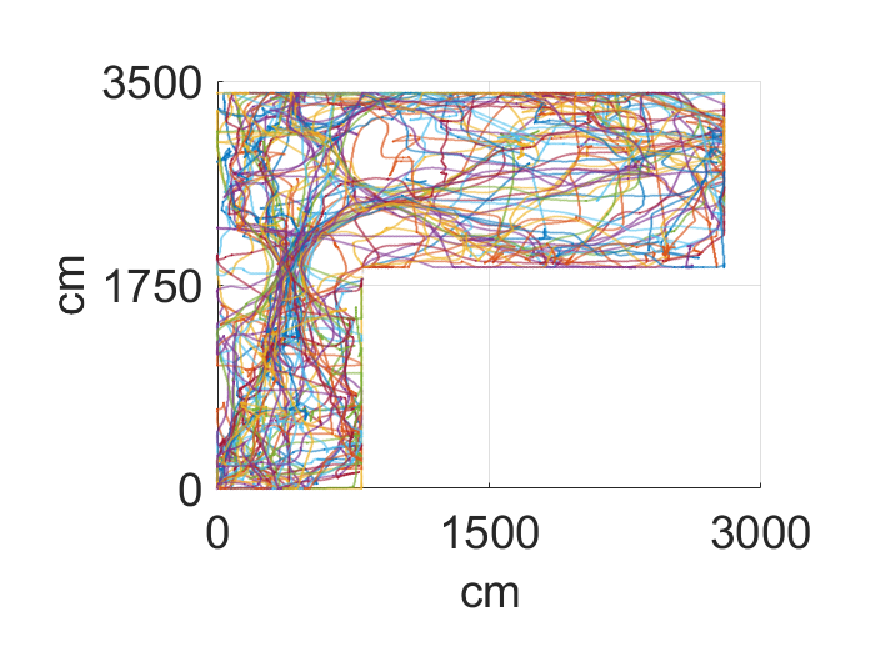
\includegraphics[width=\linewidth]{figs/firefly/museum_trajectory.pdf}
		\caption{\small Users' translational trajectories (the Museum scene).}
		\label{fig:museum_trajectory}
	\end{minipage}
	\begin{minipage}{.45\textwidth}
		\centering
		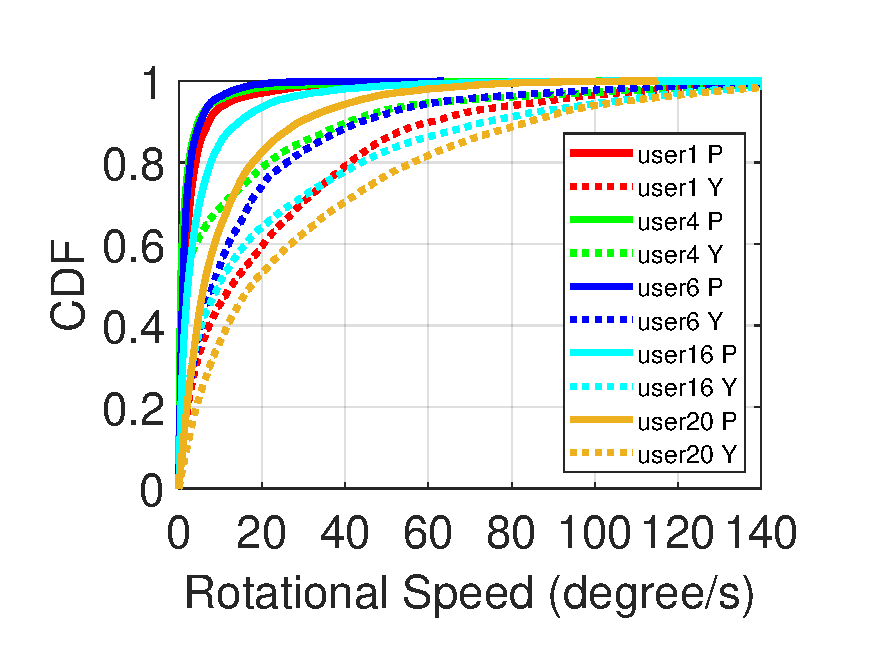
\includegraphics[width=\linewidth]{figs/firefly/angular_velocity.pdf}
		\caption{\small Five users' rotational speed (P=Pitch, Y=Yaw).}
		\label{fig:angular_velocity}
	\end{minipage}
\end{figure*}


\textbf{Collecting Viewport Movement Data from Real Users.} We conduct an IRB-approved user study involving 25 voluntary participants recruited from a large university. Among the 25 users, 9 are female. The users are from 8 departments as undergraduate (16), master (4), and Ph.D. students (5). %12 of them have prior experiences with VR.
During the study, each subject wears an Oculus Rift headset~\cite{rift} connected to a high-end PC. The subject can freely make rotational movement by moving her head as well as perform translational movement using the handheld controller.

We obtain two large VR scenes from the Unity store: Office~\cite{office} (30m$\times$26m) and Museum~\cite{museum} (35m$\times$30m, L-shape). We then develop a custom VR system (different from \firefly) that loads each scene for the users to explore. Our system logs from each user the precise viewport trajectory.
%including the viewpoint position and viewing direction.
%
We let each subject explore each scene in a random order for 5 minutes, with an arbitrarily long break allowed between the two sessions.
%
%After the study, most subjects agreed that the user experience was good, while some told us the VR headset's cable caused a bit inconvenience -- this is exactly why we need untethered VR in particular for multi-user. %Each participant received a \$20 compensation for participating our study.
We will make our dataset publicly available.

\textbf{Motion Trace Characterization.}
We now characterize the unique dataset above
%Leveraging the above unique dataset, we now present measurement results
to reveal VR users' motion dynamics and to provide insights for \firefly's design.
%
To begin with, Figure~\ref{fig:office_trajectory} and~\ref{fig:museum_trajectory} plot the translational movement trajectories of all users, represented by different colors, for the two VR scenes.
%
As shown, in most locations, the users' trajectories are highly heterogeneous.
%Similar observations are made for rotational movement trajectories (figure not shown). In contrast, prior studies have shown that for 360\DEG videos, different users oftentimes exhibit common interested regions in many frames~\cite{xx}. While the content difference may play a role, we think another reason is that compared to 360\DEG videos, generic VR includes more dimensions that increase users' motion diversity.
This finding suggests that the server should not use broadcast or multicast, simply because users typically see different content at a given time.

Fast motion may cause difficulties for viewport prediction. We thus quantify the users' motion speed.
The translational movement speed is fixed at 1m/s (set based on reported experiences from another user study)
when the user presses the controller button.
%
Figure~\ref{fig:angular_velocity} plots the distributions of rotational movement speed, calculated by sliding a 500ms window over the trajectory, across all window positions for five randomly selected users. As shown, the users exhibit different speeds, whose medians range from 1.3\degree{}/s to 18.6\degree{}/s for yaw and from 0.5\degree{}/s to 7.0\degree{}/s for pitch.
%
The median speed across all 25 users is 10.2\degree{}/s and 2.4\degree{}/s for yaw and pitch, respectively. Interestingly, such speeds match those for typical 360\degree{} users~\cite{qian2018flare}, implying
that translational movement does not necessarily slow down the rotational movement.


\begin{figure*}[t]
	\centering
	\begin{minipage}{.25\textwidth}
		\centering
		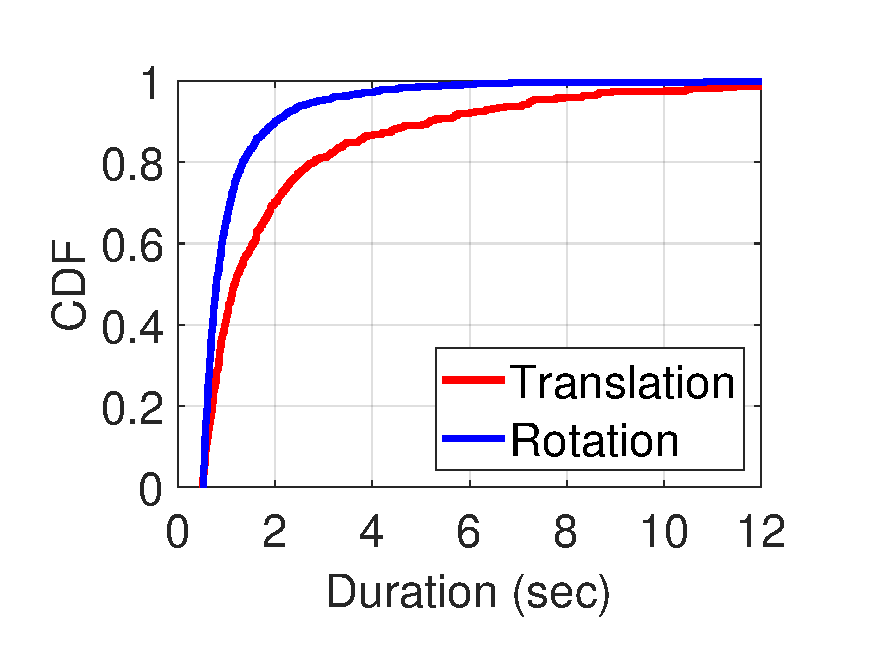
\includegraphics[width=\linewidth]{figs/firefly/per_pause_duration.pdf} \vspace{-.25in}
		\caption{\small SP\\ duration per pause.}
		\label{fig:per_pause_duration}
	\end{minipage}
	\hspace{-.1in}
	\begin{minipage}{.25\textwidth}
		\centering
		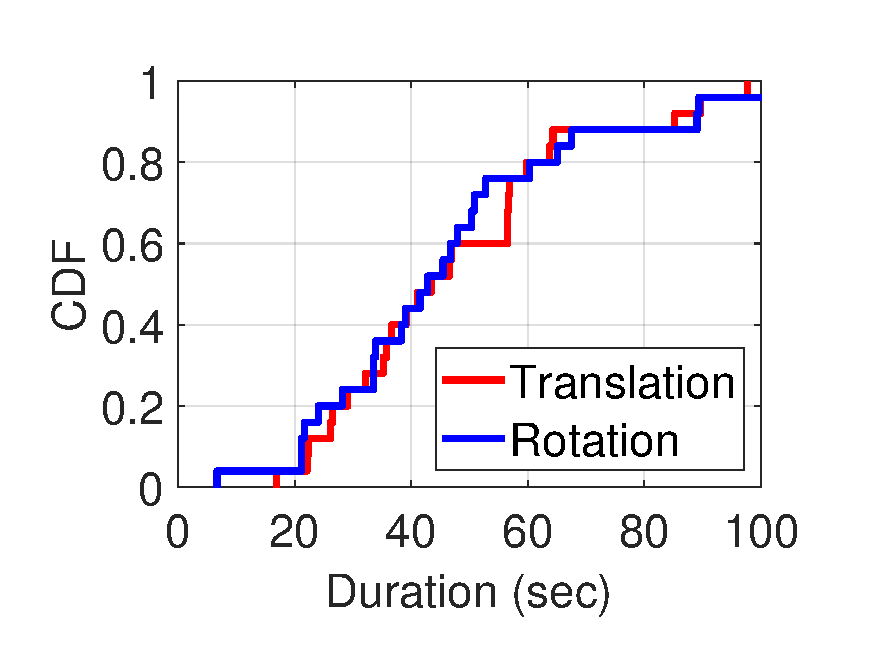
\includegraphics[width=\linewidth]{figs/firefly/total_pause.pdf} \vspace{-.25in}
		\caption{\small Total\\ SP per user.}
		\label{fig:total_pause}
	\end{minipage}
	\hspace{-.1in}
	\begin{minipage}{.25\textwidth}
		\centering
		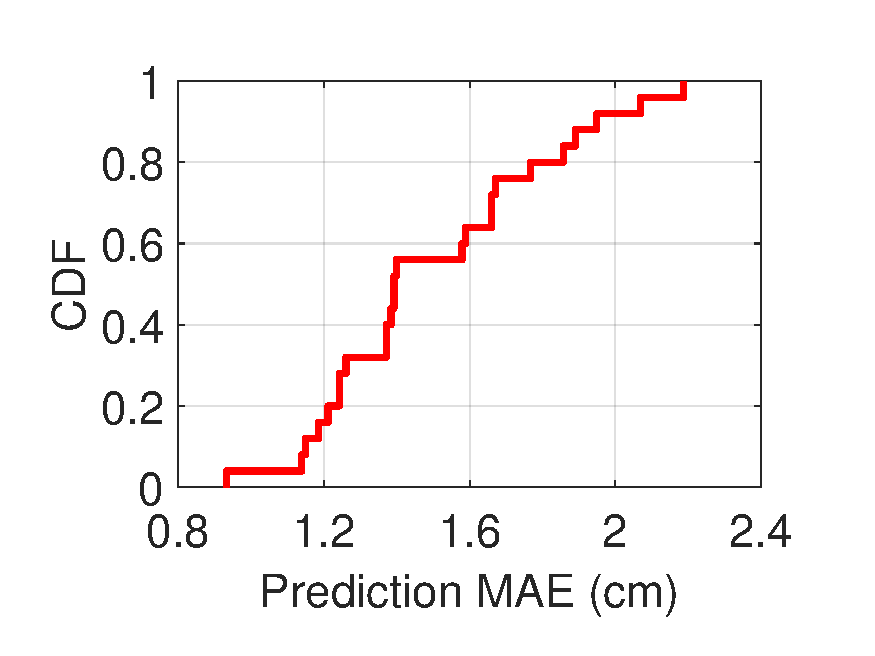
\includegraphics[width=\linewidth]{figs/firefly/translation_mae.pdf} \vspace{-.25in}
		\caption{\small Trans.\\ prediction MAE.}
		\label{fig:translation_mae}
	\end{minipage}
	\hspace{-.1in}
	\begin{minipage}{.25\textwidth}
		\centering
		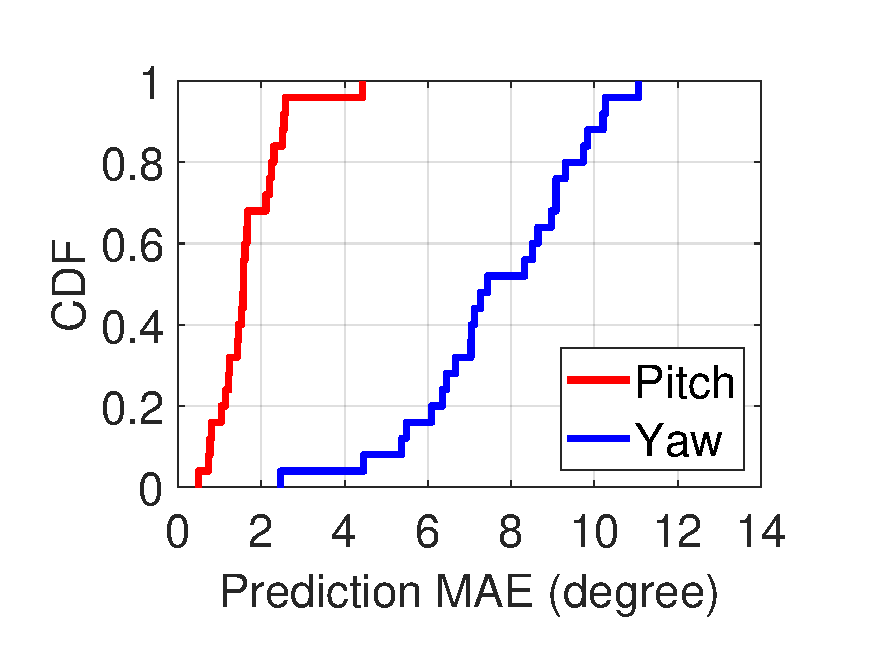
\includegraphics[width=\linewidth]{figs/firefly/rotation_mae.pdf} \vspace{-.25in}
		\caption{\small Rot.\\ prediction MAE.}
		\label{fig:rotation_mae}
	\end{minipage}
	\vspace{-.2in}
\end{figure*}


Another challenging scenario is users' sudden movement after a stationary period. How often do stationary periods (SPs) occur? Figure~\ref{fig:per_pause_duration} plots the distributions of SP duration per pause, which by our definition has to last at least 500ms. %yaw+pitch<2deg 500ms
%
Figure~\ref{fig:total_pause}  plots the total SP duration per user.
As shown, an SP is typically short: 69\% of translational SPs and 89\% of rotational SPs are shorter than 2 seconds. However, Figure~\ref{fig:total_pause} indicates that they occur frequently: within a 5-min VR session, a typical user spends 43 seconds (median) being stationary. Such frequent SPs lead to bursty, non-continuous movement patterns that pose difficulties for viewport prediction.
%
To deal with SPs, we design mechanisms such as conservative tile scheduling and bandwidth reservation (\S\ref{sec:prefetch}).
%
We also find that translational and rotational SPs are not correlated, \ie
a user is typically looking at a fixed direction while moving, or looking around while standing still.
This motivates us to separate the translational and rotational dimensions when performing viewport prediction (see below).

\textbf{Viewport (Motion) Prediction} is required by the tiling scheme.
We make two decisions regarding \firefly's viewport prediction scheme.
%
First, we decide to run it distributively on client devices to make the server scalable.
%
Second, given the above measurement results, we predict each dimension separately (yaw/pitch for rotational movement and X/Y/Z for translational movement), and then combine
them into the final predicted view. We find that this strategy greatly reduces the computational complexity while achieving a decent accuracy -- a desirable tradeoff we want to strike.
%
Regarding the actual algorithm, we continuously train a linear regression (LR) model using the motion trajectory observed within a history window of $H$ milliseconds; we then use this model to predict the future trajectory within a prediction window of $P$ milliseconds before discarding the model. The simple LR model is found to very lightweight yet effective for 360\degree{} videos~\cite{qian2018flare}; here we investigate its effectiveness for generic VR motion prediction. 
%
Ideally, $P$ should be set to the duration of the entire tile processing pipeline (form request being sent to tiles being decoded) plus some safety margin. Guided by this, we set $P$ to 150ms based on empirical profiling. We set $H$ to 50ms based on cross-validating different values of $H$, which is found to not qualitatively impact the prediction accuracy.

Figure~\ref{fig:translation_mae} and~\ref{fig:rotation_mae} plot the prediction results
for translational and rotational movement, respectively, across all users ($H$=50ms, $P$=150ms, the Office scene), with the SPs excluded.
%
The accuracy metric is the mean absolute error (MAE, in distance or degree). %The stationary periods are excluded.
The overall accuracy is high: the median MAE is around 1.4 cm for translational movement, and 1.6\degree{}/7.4\degree{} for vertical (pitch) / horizontal (yaw) rotational movement. The results for the Museum scene are similar.


\section{Future Work}
\subsection{Client-side tile fetching scheduling}
\label{sec:prefetch}
Based on the viewport prediction results, the client needs to judiciously determine which (mega) tiles
to (pre)fetch and in which order. Meanwhile, Due to users’ randomness,
viewport prediction errors are inevitable. \firefly therefore needs to apply a client-side tile (pre)fetching mechanism which also tolerates viewport prediction errors by reserving bandwidth conservatively. The design and implementation of such scheduling algorithm will be my next step.

\subsection{Adaptive quality control (AQC)}
\label{sec:aqc}
AQC takes as input the lists of tiles requested by the users,
and outputs each user’s appropriate quality level. It runs on
the server that has the global knowledge of all users. An ideal
AQC algorithm has the following features. (1) For each user,
AQC will maximize the quality level while minimizing the
stall (rebuffering); meanwhile, the number of quality switches
should be minimized to provide a smooth user experience.
(2) The selected quality levels should be fair across all the
users; in other words, the quality levels should be largely
proportional to the users’ wireless channel capacities. (3)
AQC needs to execute in a fast-paced manner (ideally at the
per-frame granularity for each user) to adapt to users’ motion.
(4) AQC should scale well for multiple users. The design and implementation of \firefly AQC module algorithm will be part of my future work.
 
\subsection{Handling dynamic foreground objects}
A VR scene may consist of a background view as well as
one or more foreground objects. The background view at
a specific virtual location is static. Due to its large area and
complexity, its rendering typically dominates the workload for
preparing the scene. In contrast, foreground objects are more
dynamic and less complex than a background scene. Their
examples include moving objects (\emph{e.g.}, other users’ avatars)
and interactive objects (\emph{e.g.}, a virtual control panel). Despite
being less complex than the background view, due to their
dynamic and interactive nature, failure to render foreground 
objects in time may also cause considerable QoE degradation. My plan on this is to design and implement an adaptive foreground objects rendering scheme. Specifically, objects’ 3D models will be distributed
to the clients offline. They are then rendered locally
by the client. This eliminates the uncertainty caused by the
network as well as the potential resource competition from
other users compared to a server-side approach. To prevent too
many objects appearing in the viewport from slowing down
client-side rendering, \firefly should support adaptively reducing the
objects’ fidelity to maintain a high FPS
